\documentclass[10pt,a4paper]{article}
\usepackage[margin=2.2cm]{geometry}
\usepackage[T1]{fontenc}
\usepackage{lmodern}
\usepackage{parskip}
\usepackage{booktabs}
\usepackage{tabularx}
\usepackage{array}
\usepackage{float}
\usepackage{needspace}
\usepackage{graphicx}
\usepackage{enumitem}
\usepackage{xcolor}
\usepackage{xurl}
\usepackage[colorlinks=true,urlcolor=blue!60!black,linkcolor=black]{hyperref}

\graphicspath{{results/graphs/}}
\newcolumntype{L}{>{\raggedright\arraybackslash}X}
\newcommand{\PM}{\ensuremath{\,\pm\,}}
\renewcommand{\arraystretch}{1.15}

\title{Post-Quantum VPN Benchmark Report\\[3pt]
\large Classical VPN vs.\ post-quantum VPN on an ESP32, measured three times}
\author{}
\date{27 November 2026}

\begin{document}
\maketitle

\section*{Summary}

We built the same VPN twice. The \textbf{classical VPN} uses X25519 and Ed25519. The
\textbf{post-quantum VPN} uses ML-KEM-512 and ML-DSA-44, which a quantum computer cannot break.
Both encrypt the data with the same AES-256-GCM code. This report compares them on an ESP32 and on the
laptop gateway. Every ESP32 and laptop test was run \textbf{three times}, and we report the
\textbf{mean of the three runs with a 95\% confidence interval}.

\begin{enumerate}[nosep]
  \item \textbf{Post-quantum costs more only when a device connects.} The handshake takes
        188\,ms instead of 86\,ms (2.2 times longer) and sends 6,562 bytes instead of 346 (19 times more).
        No handshake failed in either VPN (0 of 300 each).
  \item \textbf{After that, both VPNs cost the same.} Same added delay per message (under about
        1.3\,ms), same top speed (about 1.6\,Mbit/s), same CPU use (about 1\% in normal use, 9\% for a
        102\,kbit/s stream).
  \item \textbf{Rekeying is faster with post-quantum}: 22.5\,ms instead of 37.5\,ms.
  \item \textbf{Memory:} the post-quantum VPN uses about 63\,KB more heap. About 87\,KB is still free.
  \item \textbf{Everything is correct:} all known-answer tests pass, and our ML-KEM-512 and ML-DSA-44
        matched two independent implementations in 9,000 of 9,000 random checks, twice.
\end{enumerate}

% ---------------------------------------------------------------------------
\section{What we tested}

\begin{table}[H]\centering\small
\begin{tabularx}{\linewidth}{lLL}
\toprule
Job & Classical VPN & Post-quantum VPN \\
\midrule
Key exchange (agree on a secret) & X25519 & ML-KEM-512 (FIPS 203) \\
Signatures (prove who you are)   & Ed25519 & ML-DSA-44 (FIPS 204) \\
Encrypting the data              & AES-256-GCM & AES-256-GCM (same code) \\
Key derivation and confirmation  & HKDF-SHA256, HMAC-SHA256 & HKDF-SHA256, HMAC-SHA256 \\
Handshake                        & 4 messages, both sides sign, SA binding & same \\
\bottomrule
\end{tabularx}
\end{table}

\textbf{SA binding} means the tunnel keys and the tunnel number (SPI) are made from the session key
\emph{and} a hash of the whole handshake. If anything in the handshake was changed, the two sides get
different keys and the tunnel does not open. This version of the code is the one measured here.

\section{How we tested}

\begin{table}[H]\centering\small
\begin{tabularx}{\linewidth}{lL}
\toprule
Device & ESP32-D0WD, 2 cores at 240\,MHz. Arduino core 3.3.12, ESP-IDF 5.5.5, mbedTLS 3.6.6,
         libsodium 1.0.21, mldsa-native (low-memory setting). \\
Gateway & HP Victus 15 laptop, \textbf{charger plugged in}, \textbf{Performance} power mode,
          \textbf{Wi-Fi power saving off}. \\
Network & The laptop's Wi-Fi hotspot. The ESP32 was close to the laptop (signal $-6$ to $-19$\,dBm). \\
Runs & 3 full runs per VPN, one after the other, on 27 November 2026. \\
Statistics & Each run gives its own median (or p95). We show the mean of the 3 runs
             $\PM$ the 95\% confidence interval (Student t, $t = 4.303$ for 3 runs). \\
Units & 1\,KB = 1,024 bytes. kbps = 1,000 bits per second. \\
\bottomrule
\end{tabularx}
\end{table}

\textbf{Median and p95 in easy words.} The \emph{median} is the typical value: half of the tries were
faster, half were slower. The \emph{p95} is the slow case: 95 of 100 tries were faster than this.

\textbf{Confidence interval in easy words.} ``85.7\PM4.2\,ms'' means: our best estimate is 85.7\,ms,
and if we repeated the whole experiment, the result would very likely fall between 81.5 and 89.9\,ms.
A small interval means the runs agreed. A large one means Wi-Fi changed a lot between runs.

\subsection*{The benchmark has four parts}

\begin{itemize}[nosep]
  \item \textbf{Part A -- ESP32 (tests B0--B7):} the ESP32 runs the real VPN over Wi-Fi against the laptop
        gateway. 3 runs per VPN.
  \item \textbf{Part B -- laptop gateway (tests L0--L6):} the gateway's own speed, with fake devices on
        the laptop (no Wi-Fi). 3 runs per VPN.
  \item \textbf{Part C -- gateway crypto, in turns:} classical and post-quantum timed one after the
        other, 6 rounds, so a change in laptop speed affects both equally.
  \item \textbf{Part D -- random cross-check:} our ML-KEM-512 and ML-DSA-44 compared with two other
        implementations on 1,000 random inputs. Done twice.
\end{itemize}

A separate \textbf{signature benchmark} (Ed25519 vs.\ ML-DSA-44 alone, 100 runs, no network) is
summarised in Section~\ref{sec:sig}.

\subsection*{What each measurement means}

\begin{table}[H]\centering\small
\begin{tabularx}{\linewidth}{>{\raggedright\arraybackslash}p{3.6cm}LL}
\toprule
Measurement (KPI) & What it means in simple words & Why it matters \\
\midrule
Known-answer tests (B0, L0) & Run each algorithm on fixed inputs and compare with the official answer. & Shows the crypto is correct, not just fast. \\
AES time per KB (B1) & Time to encrypt and decrypt one message, per KB, with no network. & Cost of protecting every message. \\
Handshake time (B2) & Time from the first to the fourth handshake message. & How long a device waits before it can send data. \\
Handshake bytes (B2) & Bytes sent in the 4 handshake messages. & Matters on slow or paid radio links. \\
Failed handshakes (B2) & Handshakes that did not finish, out of 100. & Shows the VPN is reliable. \\
Added delay (B3) & Round-trip time with the VPN minus without it. & How much later a command arrives because of the VPN. \\
Top speed (B4a) & Most application data per second, 8 messages on the way. & Upper limit for data-heavy devices. \\
Steady stream (B4b) & 512\,B every 40\,ms (102.4\,kbps) for 30\,s: how much arrives and how fast replies come. & A realistic sensor or video-like load. \\
Rekey time (B5) & Time to replace the keys inside a running tunnel. & Keys are replaced every 1,000 messages or 5 minutes. \\
CPU use (B6) & How busy the ESP32's cores are. & Time left for the device's real job. \\
Heap, stack, program size (B7) & Memory the VPN uses and program size in flash. & The ESP32 has little memory. \\
Gateway crypto (L1, Part C) & Crypto time on the gateway for one handshake. & How many devices one gateway can serve. \\
Message crypto (L2) & Gateway encrypt and decrypt time per message. & Gateway cost of every message. \\
Handshake and rekey on the laptop (L3, L4) & Same as B2 and B5, without Wi-Fi. & The pure software cost. \\
Many devices at once (L5) & 1--40 devices connect at the same moment. & Behaviour when many devices start together. \\
Many tunnels open (L6) & 1--40 tunnels sending at the same time. & Gateway capacity once connected. \\
Random cross-check (Part D) & Compare with kyber-py and dilithium-py on random inputs. & Catches mistakes that fixed tests miss. \\
\bottomrule
\end{tabularx}
\end{table}

% ---------------------------------------------------------------------------
\section*{Results at a glance}
\addcontentsline{toc}{section}{Results at a glance}

All values: mean of 3 runs $\PM$ 95\% confidence interval.

\begin{table}[H]\centering\small
\begin{tabularx}{\linewidth}{Lrrl}
\toprule
What & Classical & Post-quantum & Difference \\
\midrule
Handshake time on the ESP32, median & 85.7\PM4.2\,ms & 187.6\PM9.6\,ms & 2.2 times longer \\
Handshake time on the ESP32, p95 & 144.9\PM35.0\,ms & 322.5\PM41.3\,ms & 2.2 times longer \\
Bytes sent in one handshake & 346\,B & 6,562\,B & 19 times more \\
Failed handshakes & 0 of 300 & 0 of 300 & same \\
Gateway crypto per handshake (Part C) & 0.177\,ms & 0.311\,ms & 1.8 times more \\
Added delay per message, 64\,B & +0.26\PM0.80\,ms & +0.84\PM0.32\,ms & both under 1\,ms \\
Added delay per message, 1,023\,B & +0.69\PM4.95\,ms & +1.28\PM1.15\,ms & both about 1\,ms \\
Top speed & 1,575\PM615\,kbps & 1,630\PM411\,kbps & same \\
102.4\,kbps stream delivered & 750 of 750 & 750 of 750 & same \\
ESP32 CPU: quiet / normal / stream & 0.96 / 1.14 / 8.9\% & 0.96 / 1.15 / 9.4\% & about the same \\
Rekey time on the ESP32, median & 37.5\PM4.2\,ms & 22.5\PM1.1\,ms & post-quantum faster \\
Highest heap use on the ESP32 & 126.7\PM9.0\,KB & 189.7\PM2.0\,KB & 63\,KB more \\
Heap still free & 178.6\,KB & 86.9\,KB & enough left \\
Program size & 1,021\,KB & 1,033\,KB & 12\,KB more \\
Correctness tests & all pass & all pass + 2\,$\times$\,9,000/9,000 & both correct \\
\bottomrule
\end{tabularx}
\end{table}

% ---------------------------------------------------------------------------
\section{Handshake time on the ESP32}

The post-quantum handshake takes \textbf{187.6\,ms instead of 85.7\,ms}, 2.2 times longer. Each run
timed 100 handshakes; none of the 600 failed. The three runs agreed well: 184, 187 and 192\,ms
(post-quantum) and 85, 84 and 87\,ms (classical).

Two reasons: the ESP32 must sign with ML-DSA-44, which is slower than Ed25519 and sometimes has to try
again (Section~\ref{sec:sig}); and the handshake sends 19 times more bytes over Wi-Fi. A fifth of a
second is fine for an IoT device or drone, because it connects once and keeps the tunnel open.
Connect + handshake together: 107\,ms (classical) and 210\,ms (post-quantum) typical.

\begin{figure}[H]\centering
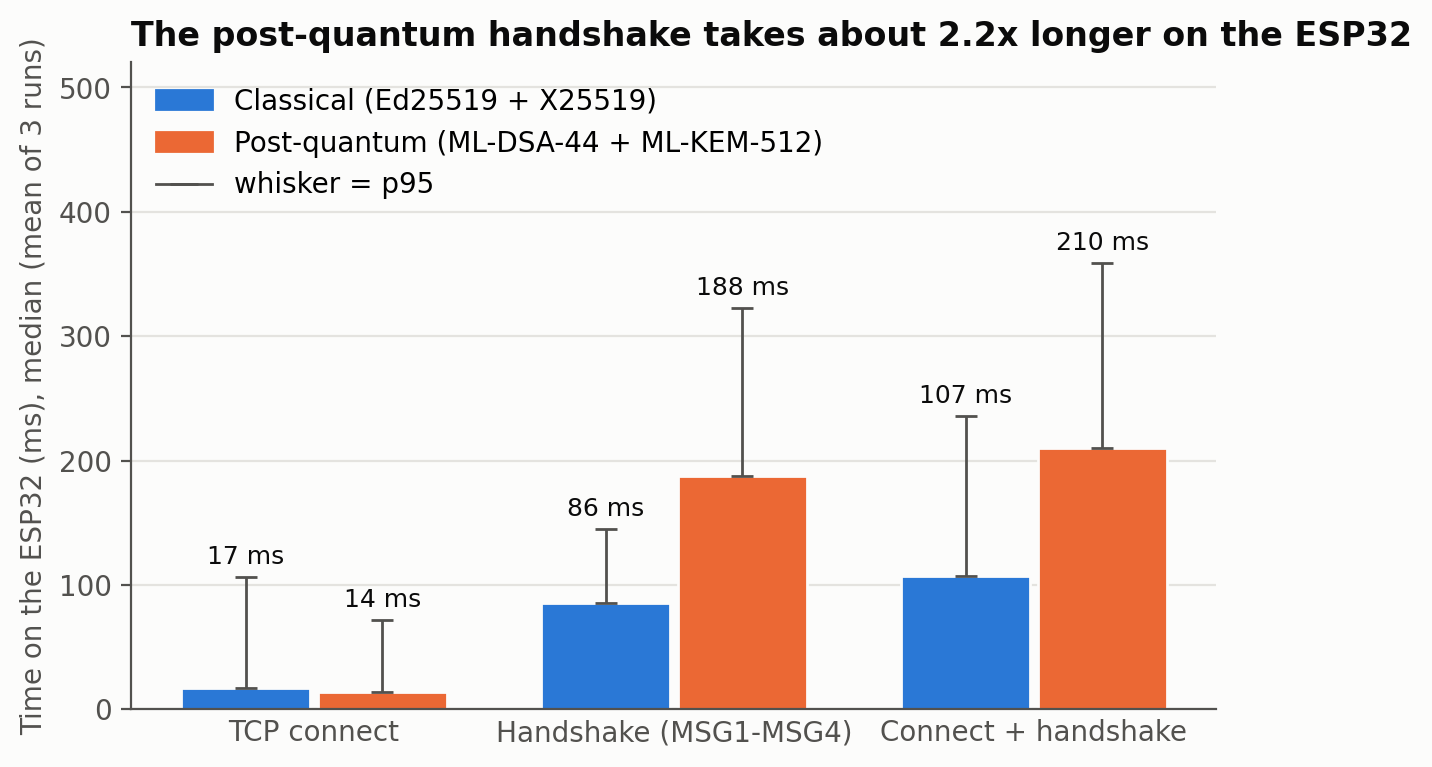
\includegraphics[width=0.75\linewidth]{1_esp32_handshake_time.png}
\caption{Handshake time on the ESP32 (mean of 3 runs, whiskers = 95\% CI).}
\end{figure}

\section{Handshake size}

The post-quantum handshake sends \textbf{6,562 bytes instead of 346}. An ML-DSA-44 public key is 1,312
bytes and a signature 2,420 bytes, against 32 and 64 bytes for Ed25519. Messages 2 and 3 carry these,
so they grow the most. Message 4 is the same 40 bytes in both: it only confirms the keys.

\begin{figure}[H]\centering
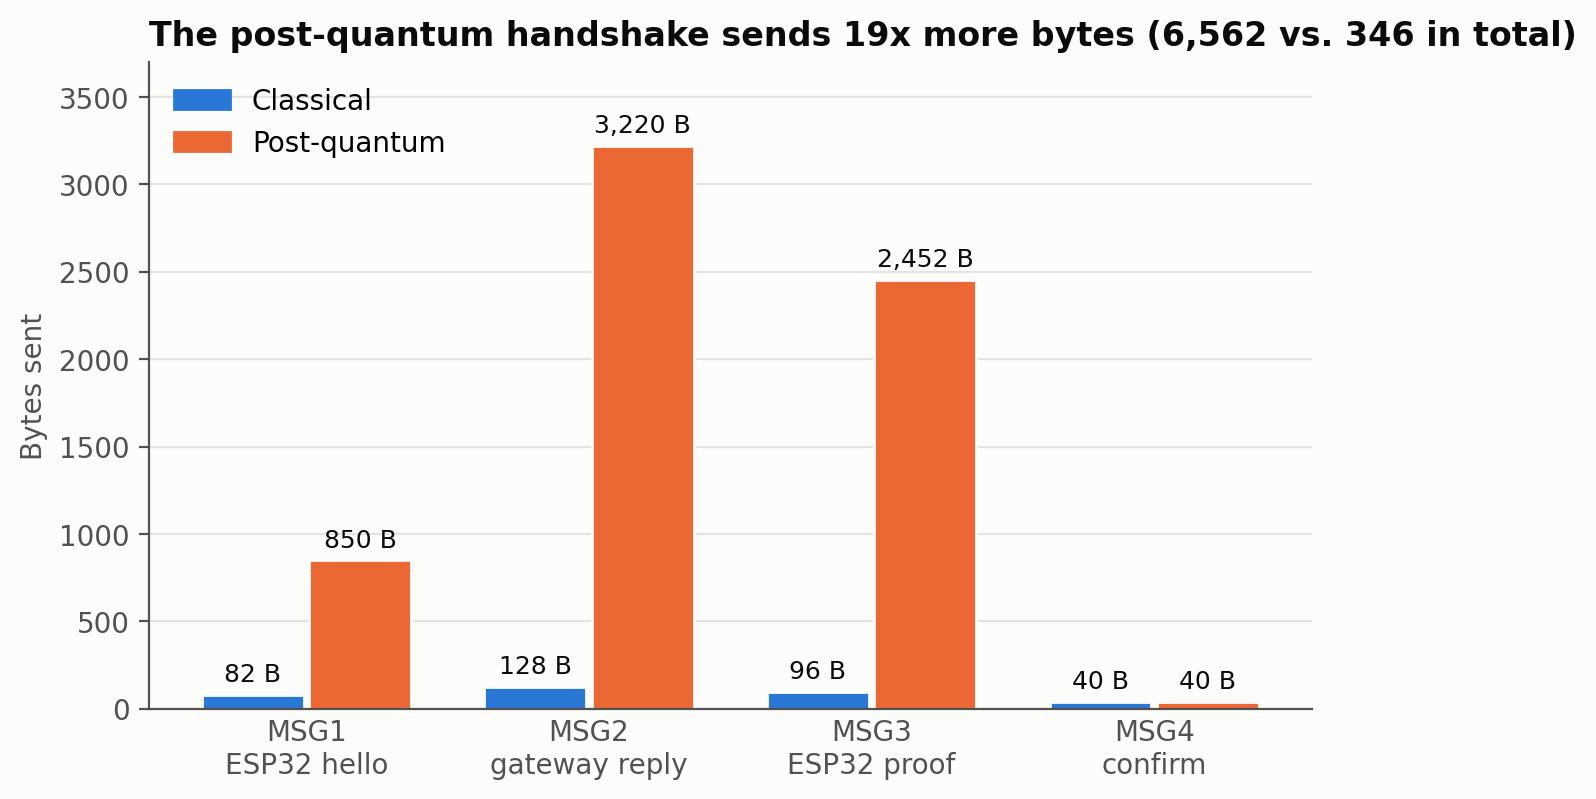
\includegraphics[width=0.75\linewidth]{2_handshake_bytes.png}
\caption{Bytes sent in each handshake message.}
\end{figure}

\section{Work done by the gateway per handshake}

The laptop gateway needs \textbf{0.311\,ms} of crypto per post-quantum handshake, against
\textbf{0.177\,ms} for classical (Part C, 6 alternating rounds of 500). Both are tiny: thousands of
handshakes per second. Only signing is slower with post-quantum (0.226 vs.\ 0.029\,ms). ML-KEM-512 is
3 times faster than X25519, and ML-DSA-44 verifies faster than Ed25519. The round-to-round spread was
1\% (classical) and 5\% (post-quantum), so the result is stable.

\begin{figure}[H]\centering
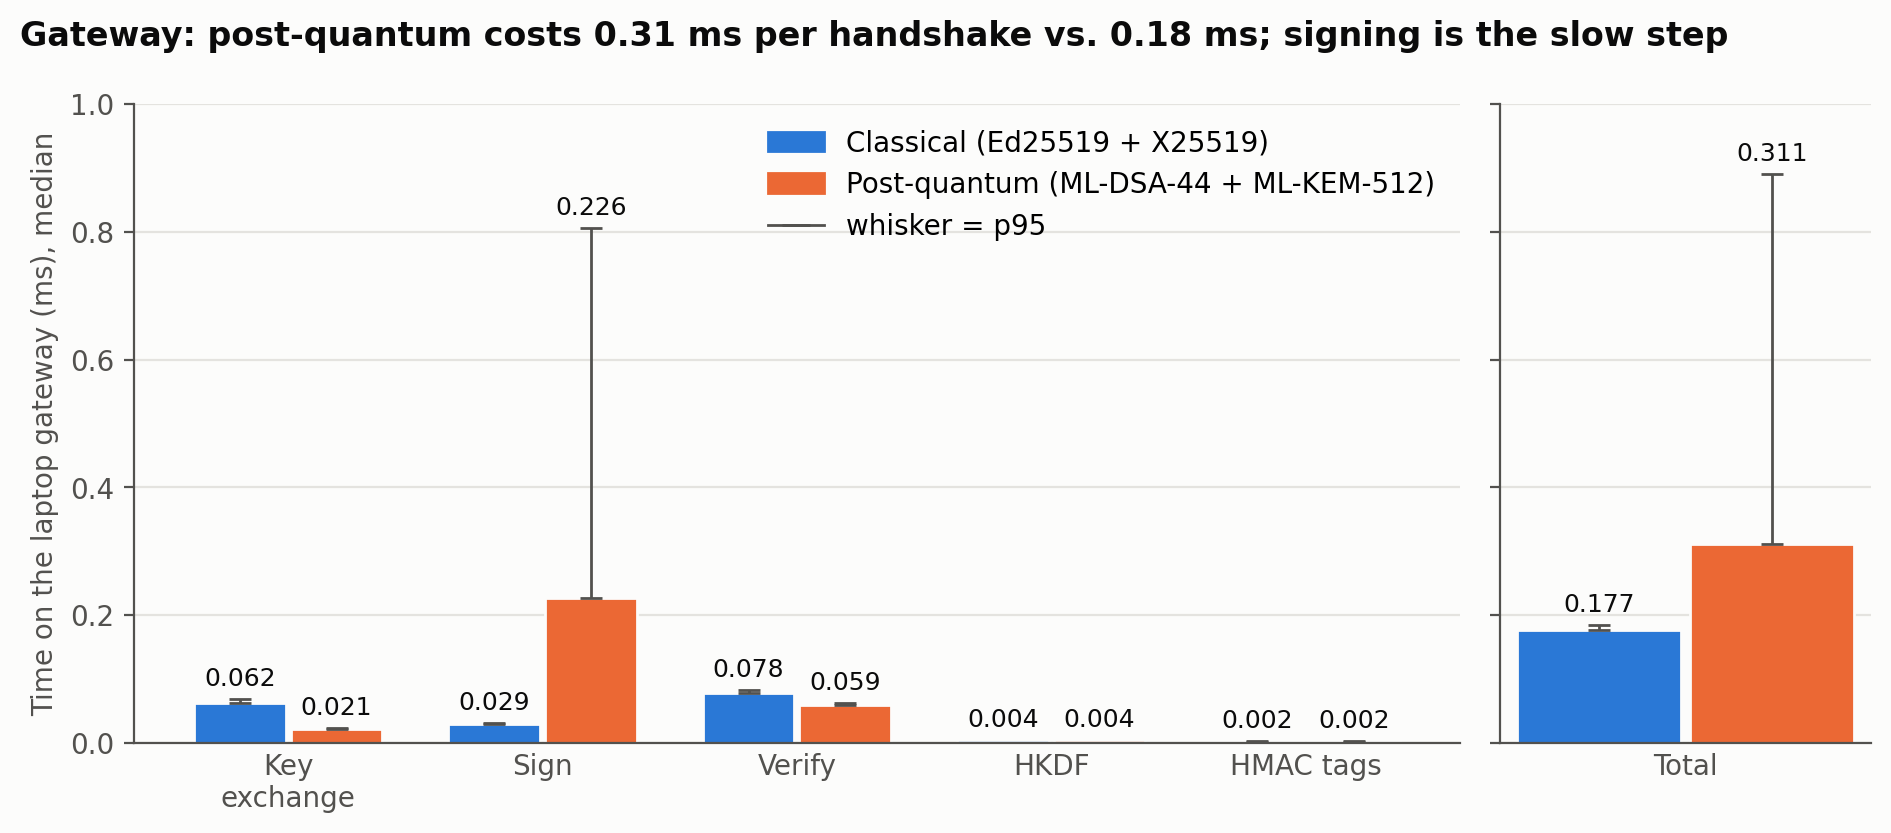
\includegraphics[width=0.9\linewidth]{3_gateway_crypto_per_step.png}
\caption{Gateway crypto per handshake, step by step (Part C).}
\end{figure}

\section{After the handshake: delay, speed and CPU}

Once connected, both VPNs cost the same, because both use the same AES-256-GCM code.

\begin{itemize}[nosep]
  \item \textbf{Added delay:} under 1\,ms for a 64-byte message and about 1\,ms for 1,023 bytes. The
        AES work itself is small (about 0.08\,ms on the ESP32 and 0.007\,ms on the laptop per 64-byte
        message); the rest is extra packet handling. The classical interval is wide because in run 2 the
        Wi-Fi happened to be slower during the plain messages than during the VPN messages, which gave a
        negative value. That is Wi-Fi noise, not the VPN being faster.
  \item \textbf{Top speed:} about 1.6\,Mbit/s for both (1,575 vs.\ 1,630\,kbps). The intervals overlap
        fully, so there is no real difference.
  \item \textbf{Steady 102.4\,kbps stream:} all 750 messages arrived in every run, for both VPNs. Typical
        reply time 10.1 vs.\ 9.3\,ms.
  \item \textbf{CPU:} about 1\% when the tunnel is quiet or in normal use, about 9\% during the stream.
\end{itemize}

\begin{figure}[H]\centering
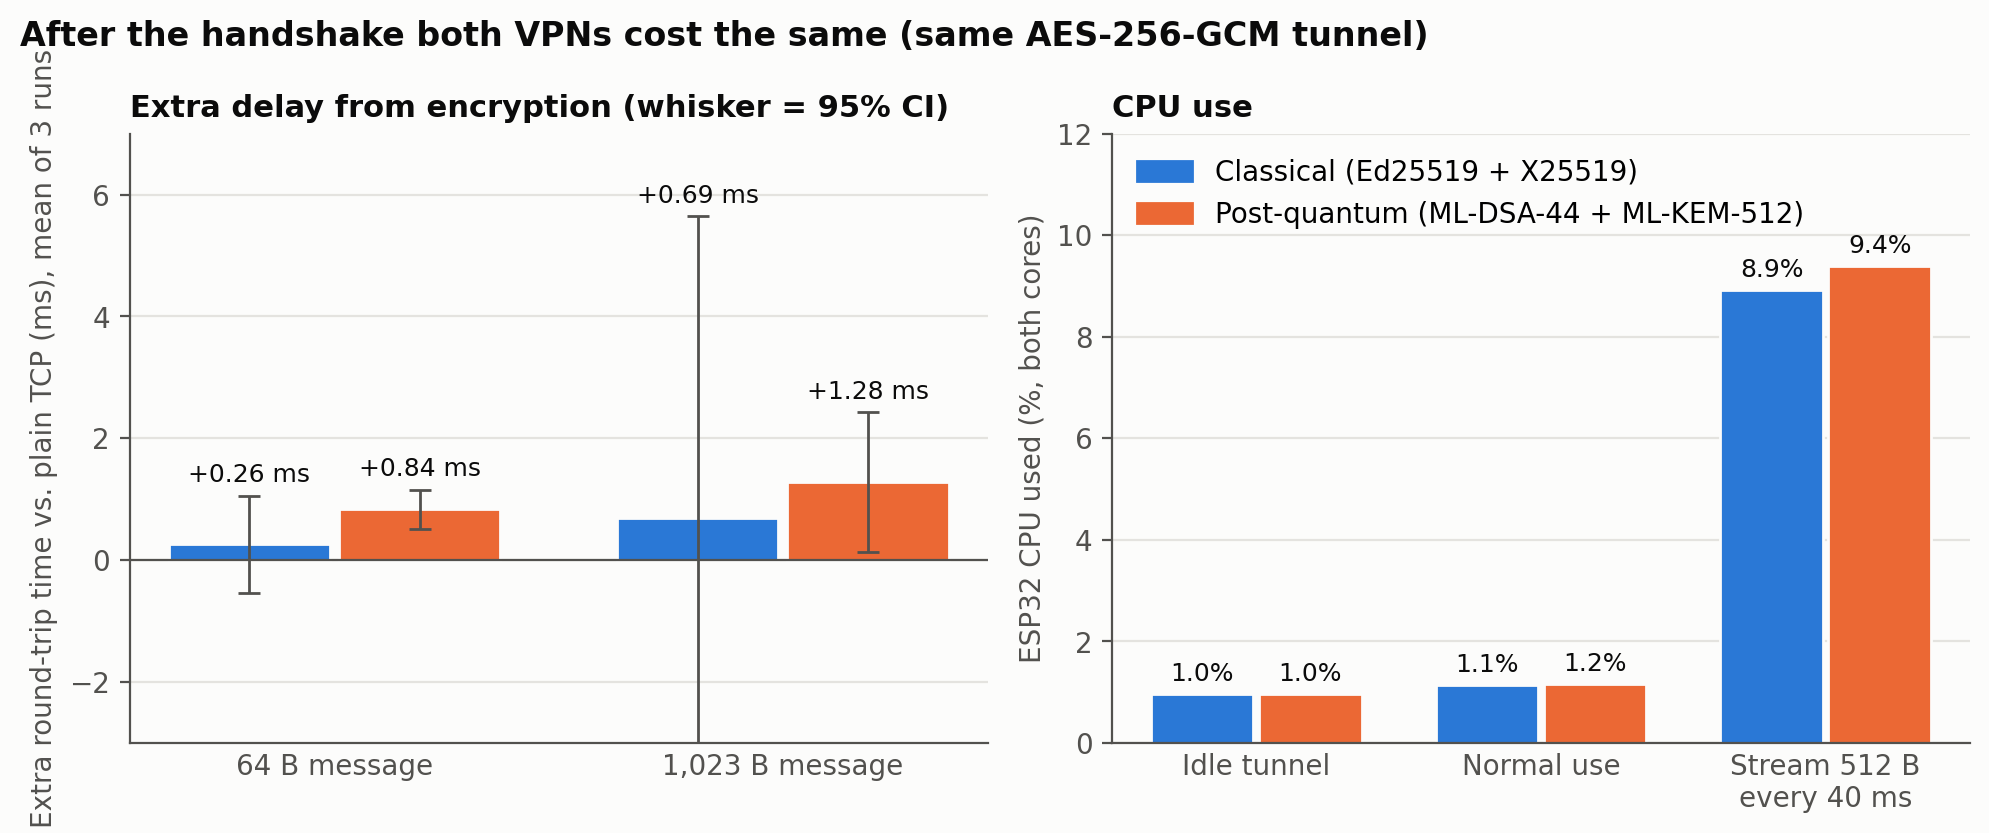
\includegraphics[width=0.95\linewidth]{4_after_handshake_latency_cpu.png}
\caption{Added delay, top speed and CPU use after the handshake.}
\end{figure}

\section{Rekeying}

Rekeying is \textbf{faster with post-quantum: 22.5\,ms instead of 37.5\,ms} (median of 20 rekeys per
run). A rekey runs a new key exchange inside the tunnel but signs nothing, and ML-KEM-512 is faster than
X25519 on the ESP32. The post-quantum rekey is also steadier (p95 26\,ms vs.\ 70\,ms).

\begin{figure}[H]\centering
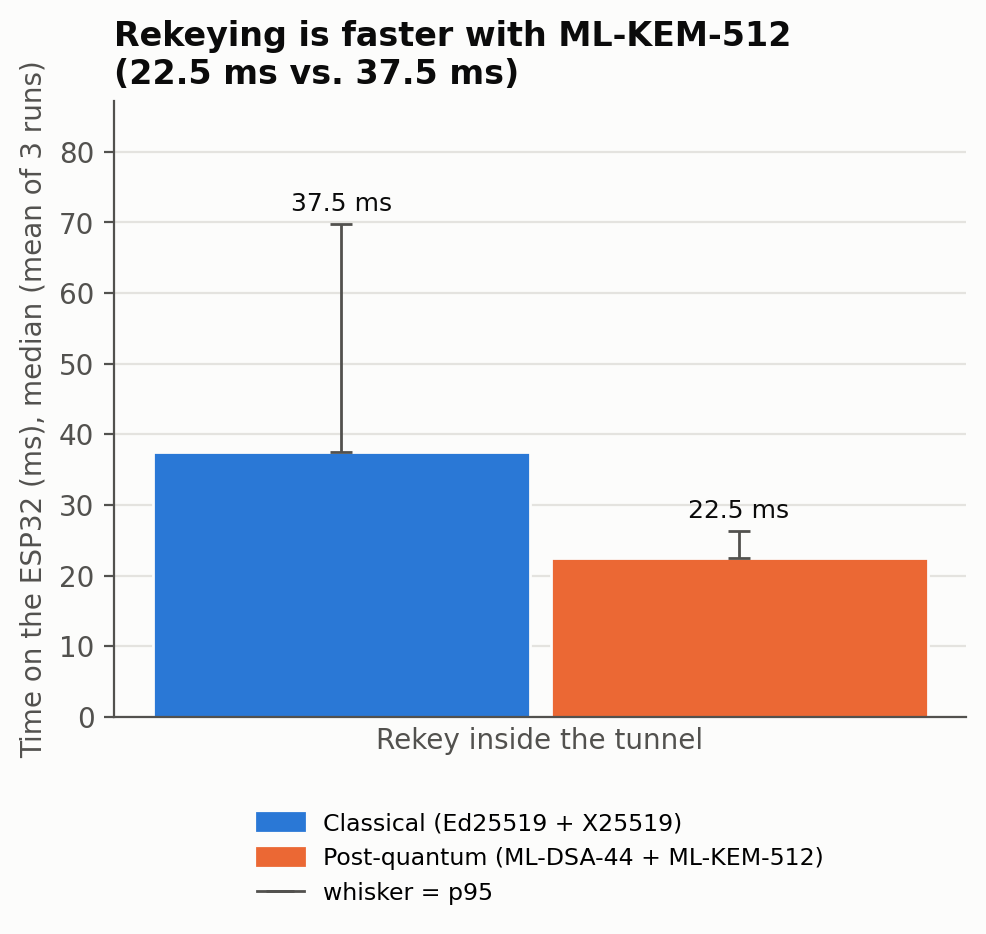
\includegraphics[width=0.45\linewidth]{5_rekey_time.png}
\caption{Rekey time on the ESP32.}
\end{figure}

\section{Memory on the ESP32}

The post-quantum VPN uses \textbf{about 63\,KB more heap} (189.7 vs.\ 126.7\,KB) and a program about
12\,KB bigger. Most of the extra heap is the 64\,KB stack of the task that runs the post-quantum code.
ML-DSA-44 signing needs about 15\,KB of stack (15,476\,B measured), and 48\,KB of that 64\,KB task stack
was never used, so the stack could be made smaller if memory gets tight. About \textbf{87\,KB of heap
is still free}, enough for the application.

\begin{figure}[H]\centering
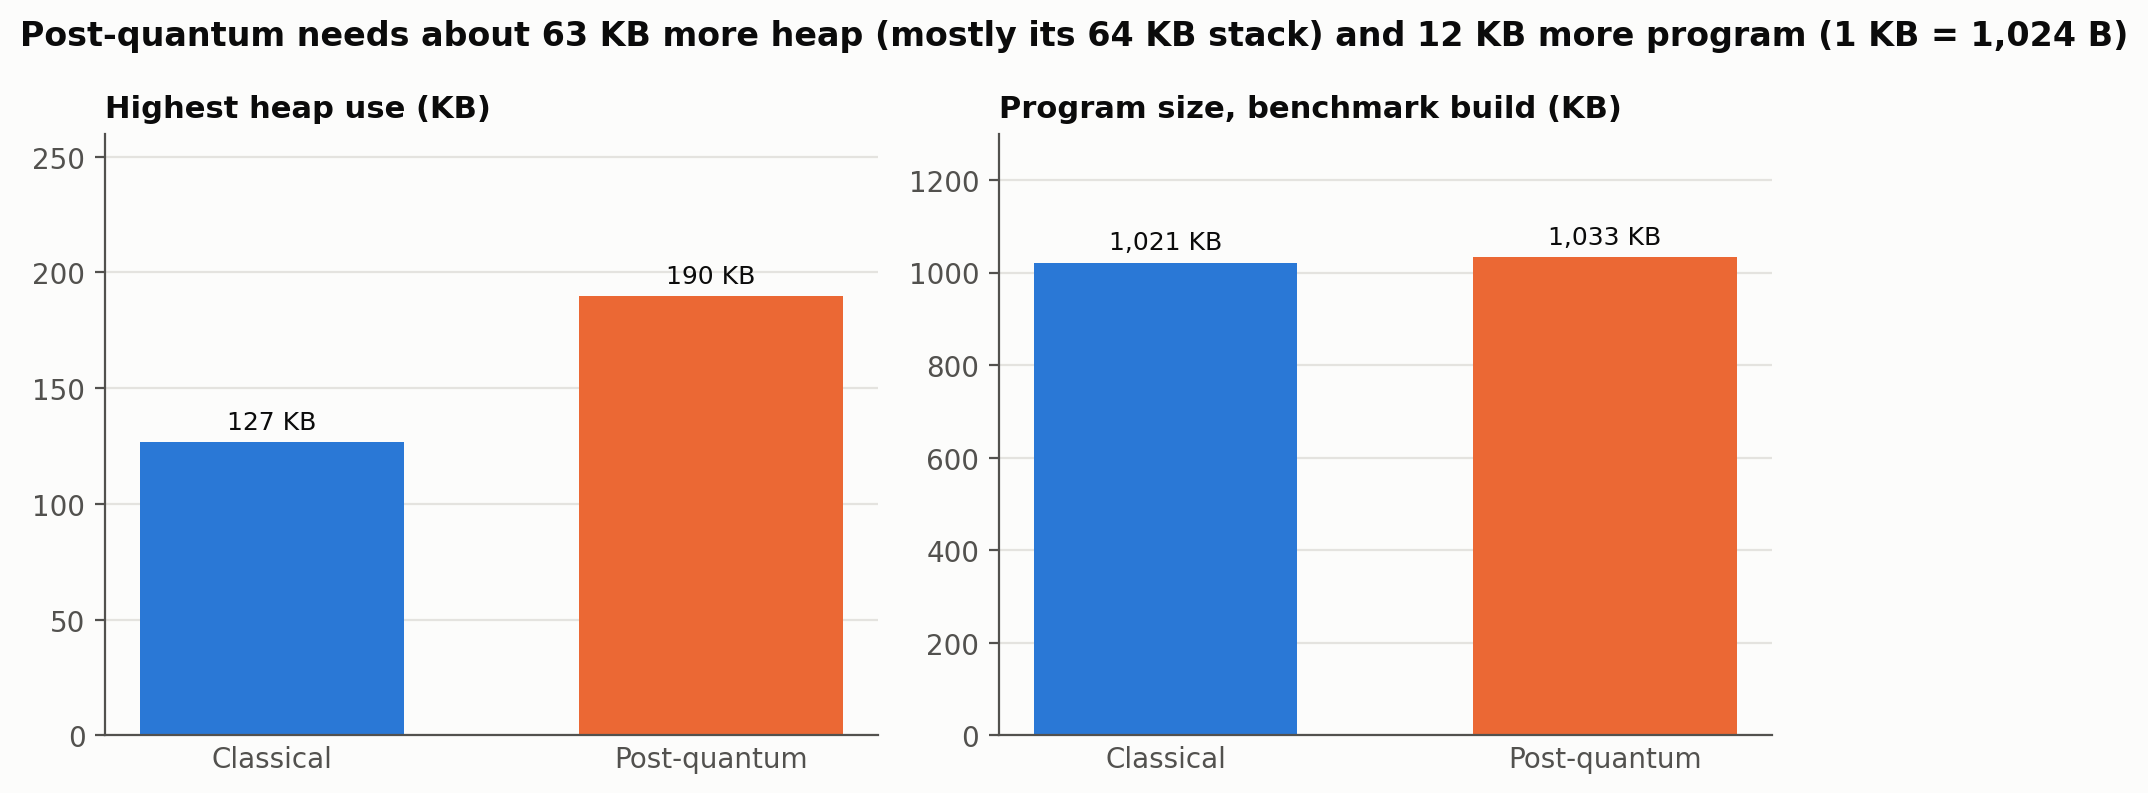
\includegraphics[width=0.95\linewidth]{6_esp32_memory.png}
\caption{Heap and program size on the ESP32.}
\end{figure}

\section{Many devices at once}

The gateway handled up to 40 devices with both VPNs, and \textbf{no connected device was ever dropped}.
These tests used fake ESP32s on the laptop.

\textbf{Devices connecting at the same moment.} To protect itself from attacks, the gateway runs at most
8 handshakes at once and tells extra devices ``busy, try again''. The post-quantum handshake takes a
little longer on the gateway, so it reaches this limit sooner: with 40 devices, on average 33.3 got in
on the first try and the rest on their next try. With classical, all 40 got in at once.

\textbf{Many tunnels open.} With 1 to 40 tunnels sending, both VPNs gave the same results: about 12,000
messages per second in total, and a reply time of about 3.3\,ms with 40 tunnels.

\begin{figure}[H]\centering
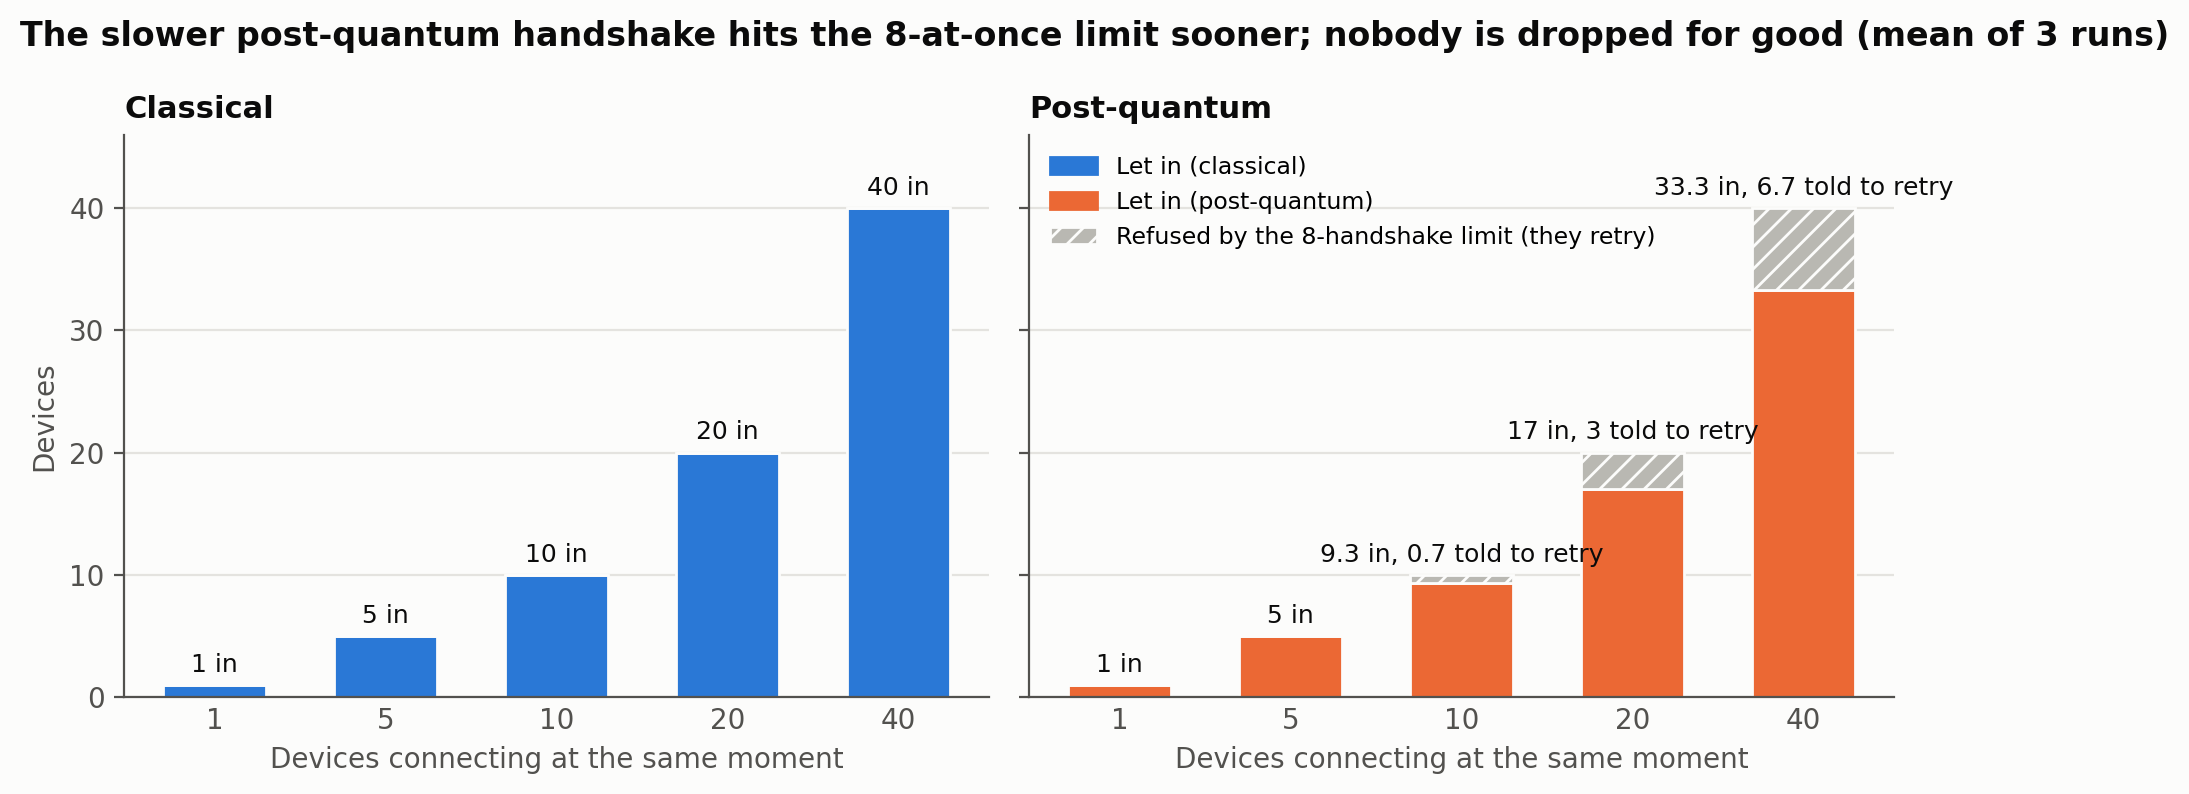
\includegraphics[width=0.95\linewidth]{7_gateway_burst.png}
\caption{Devices connecting at the same moment (L5).}
\end{figure}
\begin{figure}[H]\centering
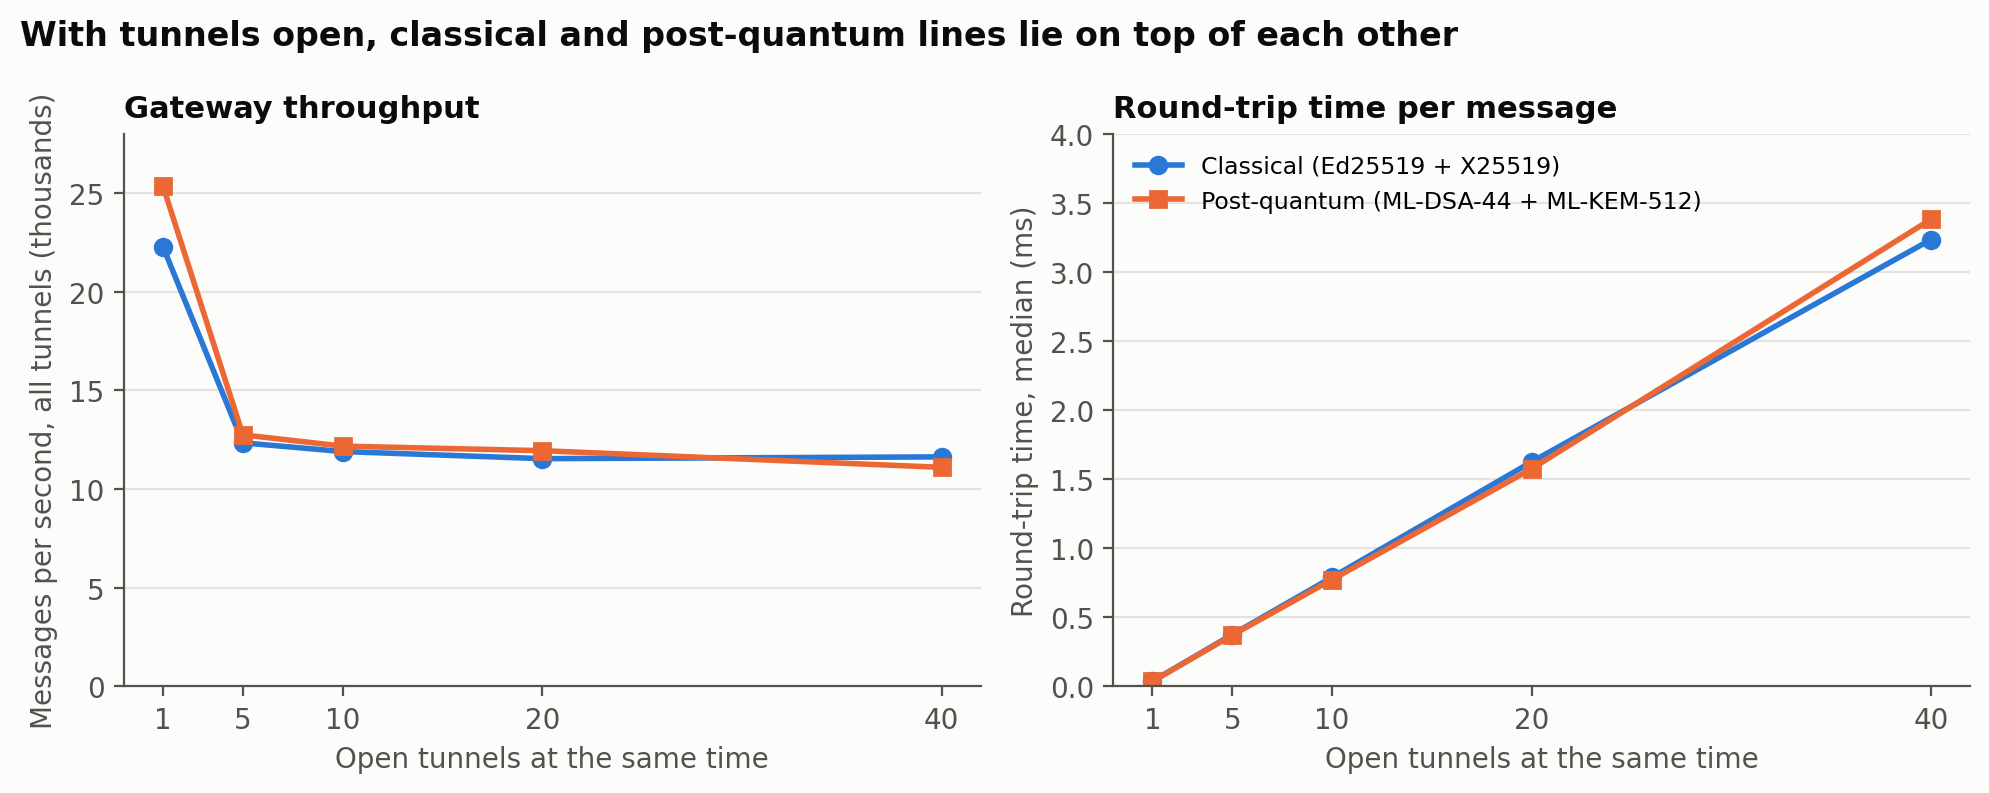
\includegraphics[width=0.95\linewidth]{8_gateway_many_tunnels.png}
\caption{Many tunnels open at the same time (L6).}
\end{figure}

\section{Are the algorithms correct?}

\textbf{Yes.} Every algorithm passed its known-answer test in every run, on the ESP32 and on the laptop.
A known-answer test runs an algorithm on fixed inputs and compares the result with a published value.
This catches mistakes that a self-test misses, because broken code always agrees with itself.

\begin{table}[H]\centering\small
\begin{tabular}{lllc}
\toprule
Algorithm & Checked against & Classical & Post-quantum \\
\midrule
SHA-256 & FIPS 180-4 example (``abc'') & Pass & Pass \\
HMAC-SHA256 & RFC 4231, test case 2 & Pass & Pass \\
AES-256-GCM & NIST GCM test case 16 & Pass & Pass \\
Ed25519 & RFC 8032, test 1 & Pass & not used \\
X25519 & RFC 7748, vector 1 & Pass & not used \\
ML-KEM-512 & kyber-py (FIPS 203) & not used & Pass \\
ML-DSA-44 & dilithium-py (FIPS 204) & not used & Pass \\
\bottomrule
\end{tabular}
\end{table}

One fixed input can miss a mistake that only happens for some inputs, so we also ran 1,000 random
tests, twice (seeds 2030312455 and 323908427). Each test compared keys, ciphertexts, shared secrets and
signatures between our code and kyber-py and dilithium-py. \textbf{All 9,000 checks were identical in
both runs.}

\section{Signature benchmark (Ed25519 vs.\ ML-DSA-44)}\label{sec:sig}

A separate sketch timed only the signatures on the ESP32: 100 runs each, no network, same libraries as
the VPN.

\begin{table}[H]\centering\small
\begin{tabular}{lrr}
\toprule
 & Ed25519 & ML-DSA-44 \\
\midrule
Make a key pair (median) & 8.40\,ms & 13.06\,ms \\
Sign (median) & 9.27\,ms & 52.94\,ms \\
Sign (mean; range) & 9.27\,ms & 77.10\,ms (20.6--487.8\,ms) \\
Verify (median) & 19.72\,ms & 13.44\,ms \\
Sign + verify (medians) & 28.99\,ms & 66.38\,ms (2.3 times) \\
Public key / signature size & 32 / 64\,B & 1,312 / 2,420\,B \\
Stack used & 3,908\,B & 15,476\,B \\
Heap used & 0\,B & 0\,B \\
\bottomrule
\end{tabular}
\end{table}

ML-DSA-44 signing \textbf{varies a lot} because it is built to try again until the signature is safe to
publish; most signatures take 20--60\,ms, a few take several hundred. This is why the post-quantum
handshake has a higher p95. Verifying is \emph{faster} with ML-DSA-44 and always takes the same time.

% ---------------------------------------------------------------------------
\section*{Full results}
\addcontentsline{toc}{section}{Full results}

Every number comes from the result files in \texttt{results/}:
\begin{itemize}[nosep]
  \item \texttt{esp32\_results\_run1.csv} to \texttt{run3.csv} and \texttt{laptop\_gateway\_results\_run1.csv} to \texttt{run3.csv};
  \item the summaries \texttt{esp32\_summary.md} and \texttt{laptop\_summary.md}.
\end{itemize}
Times are \textbf{median / p95}, each averaged over the 3 runs, unless the table says otherwise.

\subsection*{ESP32 results (Part A)}

\needspace{7\baselineskip}\textbf{B0. Known-answer tests.} Classical: 9 of 9 in every run. Post-quantum: 13 of 13 in every run.

\needspace{7\baselineskip}\textbf{B1. AES-256-GCM on the ESP32, no network (200 runs each).}
\begin{table}[H]\centering\small
\begin{tabular}{lrrrr}
\toprule
Message size & Classical: enc / dec & Post-quantum: enc / dec & Classical: per KB & Post-quantum: per KB \\
\midrule
64\,B & 0.074 / 0.073\,ms & 0.084 / 0.084\,ms & 2.37\,ms & 2.71\,ms \\
256\,B & 0.180 / 0.179\,ms & 0.190 / 0.190\,ms & 1.44\,ms & 1.53\,ms \\
1,023\,B & 0.606 / 0.606\,ms & 0.617 / 0.617\,ms & 1.21\,ms & 1.23\,ms \\
\bottomrule
\end{tabular}
\end{table}
Small messages cost more per KB because each message has a fixed setup cost. Both VPNs call the same AES
code; the post-quantum program is about 0.01\,ms slower per message because the two programs are built
differently (the code sits at different places in flash memory). This is the same in all 3 runs and
too small to matter.

\needspace{7\baselineskip}\textbf{B2. Handshake (100 handshakes per run).}
\begin{table}[H]\centering\small
\begin{tabular}{lrr}
\toprule
 & Classical & Post-quantum \\
\midrule
TCP connect & 16.7 / 106.3\,ms & 13.9 / 71.9\,ms \\
Handshake, messages 1--4 & 85.7 / 144.9\,ms & 187.6 / 322.5\,ms \\
Connect + handshake & 107.2 / 236.0\,ms & 209.9 / 358.8\,ms \\
Failed handshakes & 0 of 300 & 0 of 300 \\
Bytes sent & 346\,B & 6,562\,B \\
\bottomrule
\end{tabular}
\end{table}

\needspace{7\baselineskip}\textbf{B3. Round-trip time with and without the VPN (200 pairs per size per run).}
\begin{table}[H]\centering\small
\begin{tabular}{lrr}
\toprule
 & Classical & Post-quantum \\
\midrule
64\,B without VPN & 9.12 / 21.8\,ms & 8.71 / 15.0\,ms \\
64\,B with VPN & 9.38 / 20.8\,ms & 9.55 / 15.1\,ms \\
Added delay, 64\,B (mean $\PM$ CI) & +0.26\PM0.80\,ms & +0.84\PM0.32\,ms \\
1,023\,B without VPN & 11.97 / 26.2\,ms & 10.32 / 17.5\,ms \\
1,023\,B with VPN & 12.66 / 30.5\,ms & 11.59 / 19.0\,ms \\
Added delay, 1,023\,B (mean $\PM$ CI) & +0.69\PM4.95\,ms & +1.28\PM1.15\,ms \\
\bottomrule
\end{tabular}
\end{table}
Per run, the added delay was +0.36, $-0.10$, +0.52\,ms (classical) and +0.77, +0.99, +0.76\,ms
(post-quantum) for 64\,B. The negative value is Wi-Fi noise, not the VPN making things faster.

\needspace{7\baselineskip}\textbf{B4a. Top speed (30\,s, 1,023-byte messages, up to 8 on the way).}
\begin{table}[H]\centering\small
\begin{tabular}{lrr}
\toprule
 & Classical & Post-quantum \\
\midrule
Data delivered (per run) & 1,784 / 1,301 / 1,638\,kbps & 1,689 / 1,758 / 1,443\,kbps \\
Data delivered (mean $\PM$ CI) & 1,575\PM615\,kbps & 1,630\PM411\,kbps \\
Messages per second (mean) & 192 & 199 \\
Messages confirmed (mean) & 5,776 & 5,978 \\
Rekeys during the test (mean) & 4.7 & 4.7 \\
Failed & 0 & 0 \\
\bottomrule
\end{tabular}
\end{table}

\needspace{7\baselineskip}\textbf{B4b. Steady stream (30\,s, 512\,B every 40\,ms).}
\begin{table}[H]\centering\small
\begin{tabular}{lrr}
\toprule
 & Classical & Post-quantum \\
\midrule
Sent / delivered & 102.4 / 102.4\,kbps & 102.4 / 102.4\,kbps \\
Messages sent / confirmed & 750 / 750 & 750 / 750 \\
Reply time & 10.1 / 34.7\,ms & 9.3 / 16.8\,ms \\
\bottomrule
\end{tabular}
\end{table}

\needspace{7\baselineskip}\textbf{B5. Rekey (20 rekeys per run).} Classical 37.5 / 69.8\,ms; post-quantum 22.5 / 26.3\,ms.
Per-run medians: 39.4, 36.1, 37.1\,ms (classical) and 22.2, 23.0, 22.4\,ms (post-quantum).

\needspace{7\baselineskip}\textbf{B6. CPU use (core 0 / core 1 / average).}
\begin{table}[H]\centering\small
\begin{tabular}{lrr}
\toprule
 & Classical & Post-quantum \\
\midrule
Quiet tunnel (20\,s) & 0.65 / 1.26 / 0.96\% & 0.61 / 1.31 / 0.96\% \\
Normal use, one ping every 1.5\,s (20\,s) & 0.89 / 1.40 / 1.14\% & 0.85 / 1.46 / 1.15\% \\
Steady 102.4\,kbps stream (30\,s) & 5.05 / 12.79 / 8.92\% & 5.23 / 13.55 / 9.39\% \\
\bottomrule
\end{tabular}
\end{table}

\needspace{7\baselineskip}\textbf{B7. Memory and program size (1\,KB = 1,024\,B).}
\begin{table}[H]\centering\small
\begin{tabular}{lrr}
\toprule
 & Classical & Post-quantum \\
\midrule
Total heap & 276.7\,KB & 253.2\,KB \\
Most heap used & 126.7\PM9.0\,KB & 189.7\PM2.0\,KB \\
Heap still free & 178.6\,KB & 86.9\,KB \\
Task stack never used & 3.3\,KB of 8\,KB & 48.2\,KB of 64\,KB \\
Program size (benchmark build) & 1,021\,KB & 1,033\,KB \\
\bottomrule
\end{tabular}
\end{table}

\subsection*{Laptop gateway results (Part B)}

HP Victus 15, plugged in, Performance mode. The fake devices ran on the same laptop, so there is no
Wi-Fi delay here.

\needspace{7\baselineskip}\textbf{L0. Known-answer tests.} Classical 8 of 8, post-quantum 12 of 12, in every run.

\needspace{7\baselineskip}\textbf{L1. Gateway crypto per handshake (500 runs per run).}
\begin{table}[H]\centering\small
\begin{tabular}{lrr}
\toprule
Step & Classical & Post-quantum \\
\midrule
Key exchange (X25519 / ML-KEM-512 encapsulate) & 0.063 / 0.071\,ms & 0.021 / 0.022\,ms \\
Sign (Ed25519 / ML-DSA-44) & 0.029 / 0.033\,ms & 0.234 / 0.796\,ms \\
Verify the device's signature & 0.078 / 0.089\,ms & 0.059 / 0.061\,ms \\
HKDF session keys & 0.004 / 0.006\,ms & 0.004 / 0.004\,ms \\
Two HMAC confirmation tags & 0.0025 / 0.0026\,ms & 0.0025 / 0.0025\,ms \\
Total & 0.178 / 0.191\,ms & 0.319 / 0.881\,ms \\
\bottomrule
\end{tabular}
\end{table}

\needspace{7\baselineskip}\textbf{L2. Encrypting one tunnel message on the gateway (2,000 runs each, medians).}
\begin{table}[H]\centering\small
\begin{tabular}{lrr}
\toprule
Message size & Classical: encrypt / decrypt & Post-quantum: encrypt / decrypt \\
\midrule
64\,B & 6.5 / 6.9\,\textmu s & 6.5 / 6.8\,\textmu s \\
256\,B & 6.7 / 7.1\,\textmu s & 6.6 / 7.0\,\textmu s \\
1,023\,B & 7.2 / 7.6\,\textmu s & 7.1 / 7.6\,\textmu s \\
\bottomrule
\end{tabular}
\end{table}

\needspace{7\baselineskip}\textbf{L3 and L4. Full handshake and rekey on the laptop.}
\begin{table}[H]\centering\small
\begin{tabular}{lrr}
\toprule
 & Classical & Post-quantum \\
\midrule
L3: full handshake, both sides (100 runs) & 1.20 / 1.36\,ms & 2.31 / 3.55\,ms \\
L4: rekey, both sides (20 runs) & 0.29 / 0.34\,ms & 0.21 / 0.30\,ms \\
\bottomrule
\end{tabular}
\end{table}

\needspace{7\baselineskip}\textbf{L5. Devices connecting at the same moment} (let in on the first try, mean of 3 runs; handshake
time of those let in).
\begin{table}[H]\centering\small
\begin{tabular}{rrrrr}
\toprule
Devices & Classical: let in & Classical: handshake & Post-quantum: let in & Post-quantum: handshake \\
\midrule
1 & 1 & 1.3\,ms & 1 & 1.9\,ms \\
5 & 5 & 5.6 / 6.6\,ms & 5 & 5.5 / 6.2\,ms \\
10 & 10 & 8.9 / 12.3\,ms & 9.3 & 8.9 / 10.4\,ms \\
20 & 20 & 16.7 / 24.5\,ms & 17 & 14.5 / 19.6\,ms \\
40 & 40 & 27.6 / 46.7\,ms & 33.3 & 23.8 / 37.2\,ms \\
\bottomrule
\end{tabular}
\end{table}
Devices not let in were told ``busy, try again'' by the 8-handshake limit; none were lost.

\needspace{7\baselineskip}\textbf{L6. Many tunnels open at the same time.}
\begin{table}[H]\centering\small
\begin{tabular}{rrrrrr}
\toprule
 & \multicolumn{2}{c}{Classical} & \multicolumn{2}{c}{Post-quantum} & \\
\cmidrule(lr){2-3}\cmidrule(lr){4-5}
Tunnels & msg/s & round trip & msg/s & round trip & Dropped \\
\midrule
1 & 22,268 & 0.038 / 0.075\,ms & 25,343 & 0.037 / 0.046\,ms & 0 \\
5 & 12,340 & 0.38 / 0.68\,ms & 12,745 & 0.37 / 0.66\,ms & 0 \\
10 & 11,898 & 0.79 / 1.47\,ms & 12,172 & 0.77 / 1.43\,ms & 0 \\
20 & 11,538 & 1.63 / 3.11\,ms & 11,942 & 1.58 / 3.00\,ms & 0 \\
40 & 11,628 & 3.23 / 6.26\,ms & 11,098 & 3.38 / 6.74\,ms & 0 \\
\bottomrule
\end{tabular}
\end{table}
Messages per second is the total over all tunnels. It drops from 1 to 5 tunnels because the gateway
then shares its time between devices, and stays at about 12,000 after that.

\subsection*{Part C: gateway crypto in turns}

6 rounds of 500 timed runs each, classical and post-quantum one after the other. Medians over the rounds:
key exchange 0.062 vs.\ 0.021\,ms, sign 0.029 vs.\ 0.226\,ms, verify 0.078 vs.\ 0.059\,ms, HKDF 0.004
vs.\ 0.004\,ms, HMAC tags 0.002 vs.\ 0.002\,ms, \textbf{total 0.177 vs.\ 0.311\,ms (1.76 times)}.

\subsection*{Part D: random cross-check}

\begin{table}[H]\centering\small
\begin{tabular}{lrr}
\toprule
 & Run 1 & Run 2 \\
\midrule
Random seed & 2030312455 & 323908427 \\
Random tests & 1,000 & 1,000 \\
Checks identical with kyber-py and dilithium-py & 9,000 of 9,000 & 9,000 of 9,000 \\
\bottomrule
\end{tabular}
\end{table}

% ---------------------------------------------------------------------------
\section*{What changed since the report of 10 November 2026}
\addcontentsline{toc}{section}{What changed since 10 November}

\begin{enumerate}[nosep]
  \item \textbf{New code:} SA binding was added to both VPNs, so every test was run again on the new code.
  \item \textbf{Three runs instead of one,} with 95\% confidence intervals.
  \item \textbf{Same laptop set-up for every run:} plugged in, Performance mode, Wi-Fi power saving off.
        In the old post-quantum run the Wi-Fi was slower, which made the post-quantum top speed look
        lower (788 vs.\ 1,119\,kbps). With the same set-up, both reach about 1.6\,Mbit/s. So that
        difference came from the Wi-Fi, not the VPN.
  \item \textbf{Stack of ML-DSA-44:} the old report said signing needs about 34\,KB of stack. With the
        current library it needs about 15\,KB (15,476\,B measured).
  \item \textbf{Signature benchmark:} re-measured with the current library (Section~\ref{sec:sig}).
        The older numbers (Ed25519 signing in 15.91\,ms, ``1.9 times'') are replaced.
\end{enumerate}

The main conclusions did not change: the post-quantum handshake is about 2 times longer and 19 times
bigger, everything after the handshake costs the same, and rekeying is faster with post-quantum.

% ---------------------------------------------------------------------------
\section*{Where the benchmark code is}
\addcontentsline{toc}{section}{Where the benchmark code is}

The classical and post-quantum projects have the same benchmark files, in \texttt{Non\_PQC\_VPN/} and
\texttt{PQC\_VPN/}. Files marked ``PQC\_VPN only'' exist in one project.

\textbf{On the ESP32} (folder \texttt{esp32\_client/}):
\begin{table}[H]\centering\small
\begin{tabularx}{\linewidth}{>{\ttfamily}lLl}
\toprule
\normalfont File / function & What it does & Tests \\
\midrule
SystemBenchmark.cpp / .h & The whole ESP32 benchmark; \texttt{runSystemBenchmark()} runs every test in order and prints the versions (META lines). & B0--B7 \\
\quad benchKnownAnswer() & Known-answer tests & B0 \\
\quad benchLocalAes() & AES-256-GCM with no network & B1 \\
\quad benchHandshake() & 100 handshakes, bytes and failures & B2 \\
\quad benchLatency() & Plain vs.\ VPN round trips, one after the other & B3 \\
\quad benchThroughputMax() & Top speed, 8 messages on the way & B4a \\
\quad benchThroughputFixedRate() & The steady 102.4\,kbps stream & B4b \\
\quad benchRekey() & 20 rekeys & B5 \\
\quad benchCpuLoad(), measureCpu() & How busy both cores are & B6 \\
\quad benchMemory() & Heap, stack and program size & B7 \\
KnownAnswerTests.cpp / .h & Fixed inputs and expected answers & B0 \\
VpnLog.cpp / .h & Turns off normal printing while measuring & all \\
config.h & \texttt{BENCHMARK\_MODE} (1 = benchmark, 0 = normal VPN) and settings & all \\
\bottomrule
\end{tabularx}
\end{table}

\textbf{On the laptop} (folder \texttt{benchmarking/}):
\begin{table}[H]\centering\small
\begin{tabularx}{\linewidth}{>{\ttfamily}lLl}
\toprule
\normalfont File & What it does & Tests \\
\midrule
capture\_esp32\_bench.py & Resets the ESP32 and saves its output to \texttt{.log} and \texttt{.csv} & Part A \\
system\_benchmark/gateway\_benchmark.py -{}-serve & Gateway plus plain echo server for the ESP32 & Part A \\
system\_benchmark/gateway\_benchmark.py & Laptop tests L0--L6 & L0--L6 \\
system\_benchmark/run\_laptop\_3x.sh & Runs the laptop tests 3 times (refuses on battery) & L0--L6 \\
system\_benchmark/aggregate\_runs.py & Mean $\PM$ 95\% CI over the runs & summaries \\
system\_benchmark/compare\_gateway\_crypto.py & Gateway crypto in turns (PQC\_VPN only) & Part C \\
system\_benchmark/reference\_cross\_check.py & Random cross-check (PQC\_VPN only) & Part D \\
system\_benchmark/make\_graphs.py & The graphs in this report (PQC\_VPN only) & graphs \\
mutual\_auth\_benchmark/ & Signature benchmark sketch and graphs & Section~\ref{sec:sig} \\
\bottomrule
\end{tabularx}
\end{table}

\textbf{Results} (folder \texttt{system\_benchmark/results/}):
\begin{itemize}[nosep]
  \item \texttt{esp32\_results\_run1} to \texttt{run3} (\texttt{.csv} and \texttt{.log}) and \texttt{laptop\_gateway\_results\_run1.csv} to \texttt{run3.csv};
  \item \texttt{esp32\_summary.md/.csv} and \texttt{laptop\_summary.md/.csv} (PQC\_VPN only);
  \item \texttt{gateway\_crypto\_comparison.md}, \texttt{reference\_cross\_check.txt} and \texttt{graphs/} (PQC\_VPN only);
  \item \texttt{archive\_before\_SA\_binding/}: the earlier single runs from before SA binding.
\end{itemize}

% ---------------------------------------------------------------------------
\section*{Conclusion}
\addcontentsline{toc}{section}{Conclusion}

A post-quantum VPN works well on an ESP32. The extra cost is paid once, when a device connects: the
handshake takes about 0.1 seconds longer (188 instead of 86\,ms) and sends about 6\,KB more. After that,
the delay, speed and CPU use are the same as the classical VPN, rekeying is faster, and about 87\,KB of
memory is still free. In return, the device is protected against attackers who record traffic today and
break it later with a quantum computer.

\end{document}
